\appendix
\chapter{}

\section{学習時のパラメータ}
\label{sec:appendix_params}

%できればここの図は自分で

提案モデルの学習時のパラメータを表\ref{tab:params}に示す。また、図\ref{fig:Adam}はAdamの挙動であり、Adamにおけるパラメータについても表\ref{tab:params}に示す。

\begin{table}[h]
\label{tab:params}
\caption{}
\begin{center}
    \begin{tabular}{lr}\toprule
        パラメータ & 値 \\ \midrule
        バッチサイズ & 1 \\ 
        エポック数 & 1000 \\ 
        $\alpha$ & 0.0002 \\ 
        $\beta_1,\beta_2$ & 0.5,0.999 \\
        $\epsilon$ & $10^{-8}$ \\ \bottomrule
    \end{tabular}
\end{center}
\end{table}

\begin{algorithm}[H]
    \SetAlgoLined
    \KwData{this text}
    \KwResult{how to write algorithm with \LaTeX2e }
    initialization\;
    \While{not at end of this document}{
    read current\;
    \eIf{understand}{
    go to next section\;
    current section becomes this one\;
    }{
    go back to the beginning of current section\;
    }
    }
    \caption{How to write algorithms}
\end{algorithm}

\begin{figure}[b]
\begin{center}
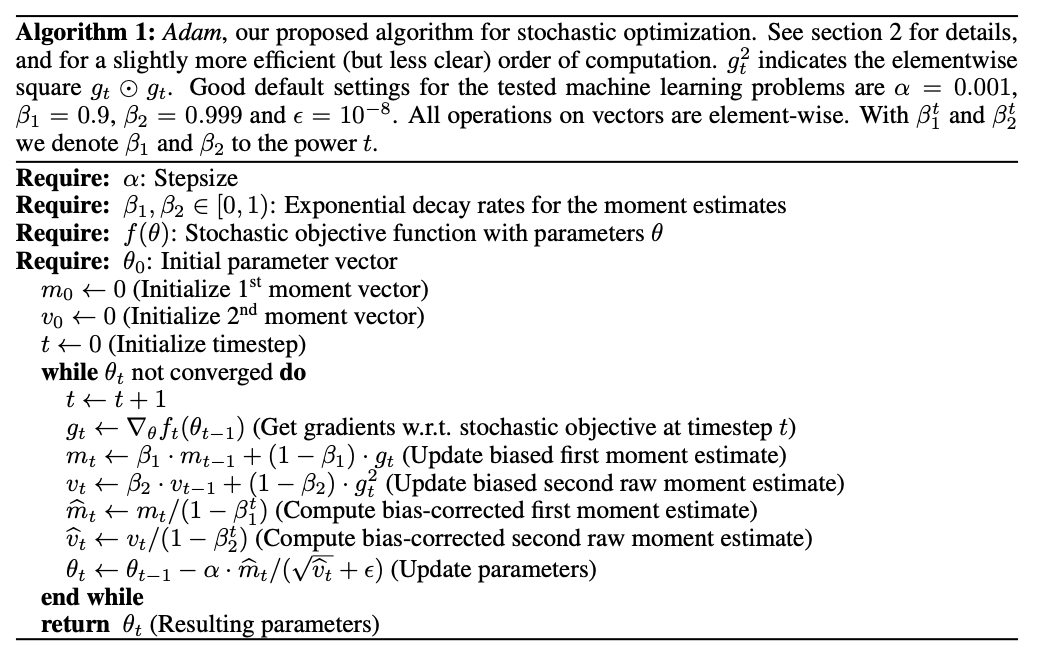
\includegraphics[width=0.9\hsize]{figure/Adam.png}
\caption{Adamの挙動\\
図は文献~\cite{Adam}より転載した。}
\label{fig:Adam}
\end{center}
\end{figure}

%ここで改ページ

\section{データセットの分割}
\label{sec:appendix_split}

生成モデルの汎化能力の評価において4分割交差検証を行ったため、図\ref{fig:data_div}のようにデータセットを4つのサブセットに分割した。また、88音をシャッフルして配列に格納した後に22音ずつ順に選ぶことで、データセットを4つに分割した。

\begin{figure}[t]
\begin{center}
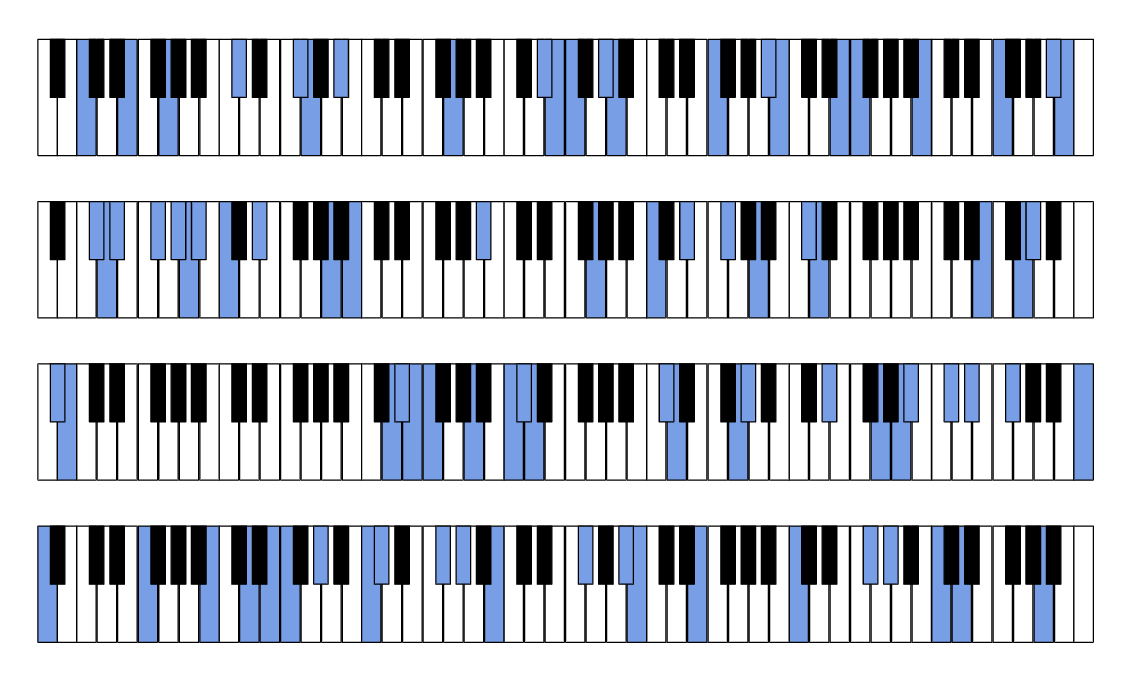
\includegraphics[width=\hsize]{figure/data_div.png}
\caption{データセットの分割方法}
\label{fig:data_div}
\end{center}
\end{figure}

\begin{comment}
\begin{table}[h]
\label{tab:split}
\caption{}
\begin{center}
    \scalebox{0.7}{
    \begin{tabular}{l|llllllllllllllllllllll}\toprule
        番号  \\ \midrule
        0 & C1 & E1 & G1 & C2$\sharp$ & F2$\sharp$ & G2 & A2$\sharp$ & G3 & D4$\sharp$ & E4 & F4 & G4$\sharp$ & A4 & F5 & A5$\sharp$ & B5 & E6 & F6 & B6 & F7 & A7$\sharp$ & B7\\ 
        1 & C1$\sharp$ & D1 & D1$\sharp$ & F1$\sharp$ & G1$\sharp$ & A1 & A1$\sharp$ & C2 & D2$\sharp$ & A2 & B2 & A3$\sharp$ & G4 & C5 & D5$\sharp$ & F5$\sharp$ & A5 & C6$\sharp$ & D6 & E7 & G7 & G7$\sharp$ \\ 
        2 & A0$\sharp$ & B0 & D3 & D3$\sharp$ & E3 & F3 & A3 & C4 & C4$\sharp$ & D4 & C5$\sharp$ & D5 & G5 & G5$\sharp$ & D6$\sharp$ & G6 & A6 & A6$\sharp$ & C7$\sharp$ & D7$\sharp$ & F7$\sharp$ & C8 \\ 
        3 & A0 & F1 & B1 & D2 & E2 & F2 & G2$\sharp$ & C3 & C3$\sharp$ & F3$\sharp$ & G3$\sharp$ & B3 & F4$\sharp$ & A4$\sharp$ & B4 & E5 & C6 & F6$\sharp$ & G6$\sharp$ & C7 & D7 & A7 \\ \bottomrule
    \end{tabular}
    }
\end{center}
\end{table}
\end{comment}